\section{基于邻域与原型的分类}
\label{sec:classification-neighborhood}

前面的线性分类器用一组全局权重决定边界。如果同一类别分布在几个相隔的区域，一条直线可能无法把它们同时与另一类分开——一个类在平面上分成两团、另一类夹在中间时，任何直线都会把其中一团划错。我们也可以暂不规定整条边界的形状，而在新输入附近寻找带标签的样本，用这些局部记录判断类别。这背后是一条与全局模型完全不同的信念：不假设存在一组统一的参数，只假设“输入靠得近，类别也倾向于相同”。这是$k$-NN分类的做法：保存训练实例，按距离找出邻居，再聚合标签。与回归中的响应平均相比，分类采用多数投票或局部类别比例。近邻表示和检索的基础见第\ref{sec:classic-overview-neighborhood}节，回归对应形式见第\ref{sec:regression-knn}节。

\subsection{k近邻分类}
\label{sec:classification-knn}

局部比较避开了预先选择全局边界，却留下一个问题：附近只取一个样本，还是让多个样本一起判断？最近的样本也可能带有噪声标签；增加邻居能平均这种波动，但范围过大又会把别处的类别混进来。近邻数因此决定了我们用多大范围的标签来描述当前输入。

\subsubsection{模型结构}
\label{sec:classification-knn-structure}

给定训练集$D_n=\{(\bm{x}_i,y_i)\}_{i=1}^n$、距离$\rho$以及$1\leq k\leq n$，用$N_k(\bm{x})\subseteq\{1,\ldots,n\}$表示查询$\bm{x}$的$k$个最近邻索引。预测规则为
\begin{equation}
  \hat h_{n,k}(\bm{x})
  =\argmax_{c\in\{1,\ldots,C\}}
  \sum_{i\in N_k(\bm{x})}\mathbb{1}\{y_i=c\}.
  \label{eq:classification-knn-vote}
\end{equation}
距离相同时，按预先约定、独立于标签的顺序选取邻居；类别票数并列时也使用固定规则。多分类在奇数$k$时也可能出现票数并列，因此两种平局都需要明确规则。

式\eqref{eq:classification-knn-vote}也可以理解为估计查询附近的类别比例：
\begin{equation}
  \hat\eta_{n,c}(\bm{x})
  =\frac{1}{k}\sum_{i\in N_k(\bm{x})}\mathbb{1}\{y_i=c\},
  \qquad
  \hat h_{n,k}(\bm{x})=\argmax_c\hat\eta_{n,c}(\bm{x}).
  \label{eq:classification-knn-posterior}
\end{equation}
比例估计解释了投票为什么可能有效：若邻域内的条件类别分布变化不大，邻居标签就能提供关于当前输入的统计证据。局部比例的误差取决于邻域大小与标签噪声，概率质量需通过样本外数据检验。

图~\ref{fig:classification-knn-neighborhood}固定训练点和查询，只改变参与投票的近邻数。取查询$\bm{x}=(0,0)$，样本1、3、4、6属于类1，其余样本属于类2。按欧氏距离计算，七个样本到查询的平方距离依编号为$1,2,2.5,4.25,5,9,10.25$，因此编号也表示由近到远的次序。

$k=1$时只有样本1投票，查询被判为类1；$k=5$时样本1至5投票，其中类1有三票、类2有两票，预测仍为类1。两幅图中的圆分别经过第1和第5个邻居，半径为$1$和$\sqrt5$。圆表示当前查询的证据范围，整个平面上的分类边界则由各查询的投票共同决定。比较两个$k$的准确性还需要查询的真实标签。

\begin{figure}[htbp]
  \centering
  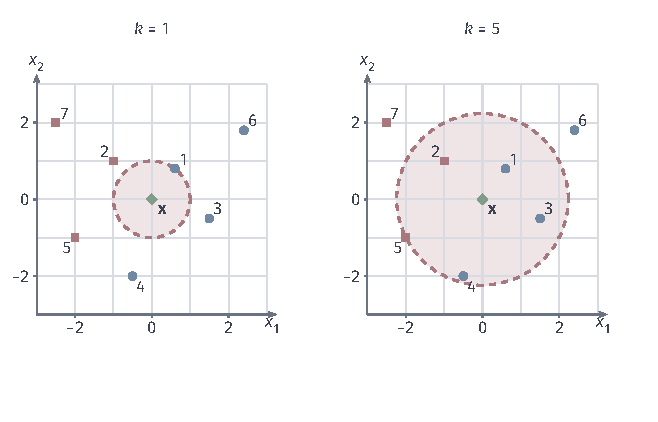
\includegraphics[width=111.404mm]{figures/04-classic-models/00-shared/tikz/classification-knn-neighborhood/figure.pdf}
  \caption{同一查询下的近邻范围与投票变化。教学构造取$n=7$、$d=2$、无量纲坐标和欧氏距离，查询为$\bm{x}=(0,0)$；两图的样本、编号及坐标尺度完全相同。蓝色圆点表示类1，红色方点表示类2，绿色菱形表示查询，红色虚线圆表示包含边界的近邻范围。左图$k=1$、半径$1$，蓝、红票数为$1:0$；右图$k=5$、半径$\sqrt5$，票数为$3:2$，因此判为蓝色类。各邻居等权投票，距离和票数均无并列；点的位置、标签与参数均为人为设定，不代表真实数据实验。}
  \label{fig:classification-knn-neighborhood}
\end{figure}

\paragraph{新查询的检索代价}
对一个新输入$\bm{x}$，预测的实际开销是把它与训练集比较、取出$k$个最近邻再投票。对$d$维稠密查询，朴素扫描$n$个训练样本计算距离需$O(nd)$；若再把所有距离排序，总代价为$O(nd+n\log n)$。采用线性选择算法得到最小的$k$项再作投票，可达$O(nd+n+k)$；使用大小为$k$的堆则需$O(nd+n\log(k+1)+k)$。因此，通常所说的$O(nd)$朴素预测复杂度隐含了无需完整排序的选择方法。训练集的存储为$O(nd)$，批量计算、硬件、精度要求和延迟预算共同决定这种实现的可用规模。给定训练得到的$D_n$、$\rho$与$k$，投票规则本身不变，改变的只是这$k$个邻居用多快的方式找出。

\subsubsection{参数学习}
\label{sec:classification-knn-learning}

\paragraph{距离与近邻配置的学习}
基本$k$-NN分类没有固定维数参数的优化过程，但需要确定输入表示、距离、近邻数及检索方式。“非参数化”是指预测关系不局限于一个固定有限维参数族；它仍有超参数，预处理和模型选择也属于学习。

距离决定哪些样本会参与投票。对数值特征，欧氏距离$\rho(\bm{x},\bm{z})=\lVert\bm{x}-\bm{z}\rVert_2$容易计算，却会放大数值范围较大的坐标。收入和年龄共同作为特征时，直接使用原始单位会让收入差异主导距离。标准化、按业务意义设定尺度或学习特征权重都可改变这一点；不同特征的重要性可通过任务知识或训练数据确定。标准化参数只能从训练集估计，交叉验证时应在各训练折内重新拟合，避免验证信息提前进入距离。

类别型特征可采用\term{汉明距离}（Hamming distance），按不同取值的坐标数比较，而不能把任意类别编码的数字差当成有意义的远近。文本的TF--IDF等稀疏向量常比较余弦相似度，强调方向而非长度；$1$减余弦相似度一般不满足三角不等式，不能直接套用所有度量空间结论。对非零向量作单位长度归一化后，按余弦相似度排序与按欧氏距离排序等价，此时可用欧氏空间中的解释。

若特征之间相关，可以考虑\term{马氏距离}（Mahalanobis distance），用协方差调整方向上的尺度：
\begin{equation}
  \rho_{\mathrm{M}}(\bm{x},\bm{z})^2
  =(\bm{x}-\bm{z})^\top
   \bm{\Sigma}^{-1}(\bm{x}-\bm{z}),
  \label{eq:classification-mahalanobis}
\end{equation}
其中$\bm{\Sigma}\in\mathbb{R}^{d\times d}$须正定。样本不足时协方差估计可能奇异，需要正则化；整体协方差也不一定符合分类所需的相似性。

近邻数$k$控制局部平均的范围。$k=1$时，一个错误标签就会影响邻近查询；增加邻居可平均这类波动，也会混入更远区域并削弱局部细节。因此$k$的选择需要结合类别比例、局部密度与距离表示，在训练集内部验证。最终选择依据相同评价条件下的误差。

\paragraph{索引构造与存储准备}
k近邻本身不训练参数，但部署前可以为训练集建立索引。KD树或球树（ball tree）等精确索引通过空间划分把训练样本组织成树，查询时排除不可能更近的样本；低维且分布有利时它们可以减少访问量，最坏情形仍会检查大部分样本。索引保留原预测规则，选择时比较建索引成本、内存和实际查询时间，维数的影响需结合数据分布测量。

高维大规模数据还可以用\term{近似最近邻检索}（approximate nearest-neighbor search）建立近似索引，查询时减少访问量；但此时返回的邻居集合可能与精确检索不同，须同时检查邻居召回率与最终分类错误。

\subsubsection{理论分析}
\label{sec:classification-knn-theory}

\paragraph{单邻居的标签随机性}
距离很近并不表示标签必然相同。记真实局部类别概率为$\eta_c(\bm x)=\mathbb P(Y=c\mid\bm X=\bm x)$；若最近邻的位置逐渐接近查询，且这些概率在该处连续，邻居标签和新样本标签仍相当于从这组概率中各抽取一次。因此，极限局部错误为
\[
  r_{1,\infty}(\bm x)=1-\sum_{c=1}^C\eta_c(\bm x)^2.
\]
平方项表示两次独立抽取都落在同一类别的概率。例如两类后验处处为$(0.8,0.2)$，此时一个“知道真实后验”的最优分类器始终选类1，错误率就是较小类的概率$0.2$；1-ND并不做这种平均，它只听信距离最近的那一个邻居的标签，而邻居的标签相当于从$(0.8,0.2)$里随机抽一次，可能恰好抽到那$20\%$的少数类。计算得$1-0.8^2-0.2^2=0.32$，正好是“新样本与最近邻这两次独立抽取落在不同类别”的概率$2\times0.8\times0.2$。也就是说，即使近到噪声可以忽略，单邻居仍要为标签本身的随机性付一次“抽样”代价，而多数投票正是靠增加邻居数来摊薄这次代价。Cover与Hart的渐近分析刻画了这项单邻居噪声；它不是任意有限训练集上的风险保证\scite{coverhart1967}。

\paragraph{增长邻域的一致性条件}
增加$k$可以平均标签波动，但同时扩大了取证范围。在固定有限维欧氏空间、独立同分布抽样、精确检索及与标签独立的距离平局处理下，若$k=k_n\to\infty$且$k_n/n\to0$，近邻分类的期望风险趋于贝叶斯风险。这里“期望”同时平均训练抽样和独立查询；Stone的一般一致性结果不要求逐点连续的后验，但证明依赖欧氏覆盖性质\scite{stone1977consistent}。这解释了为什么要同时增加票数、控制邻域范围；它不替有限样本选定一个最佳$k$，也不直接覆盖任意近似索引。

\subsubsection{距离加权投票：调节邻居影响}
\label{sec:classification-knn-weighted}

等权投票把选中的邻居一视同仁，却没有使用它们距离查询的差别。例如，在一个教学构造中，三个邻居的距离依次为$0.1$、$0.9$、$1$，最近者属于类1，另外两者属于类2。等权投票选择类2；如果我们认为近处标签更能反映查询的类别，就可以让远处两票的影响小一些。\term{加权$k$近邻}（weighted $k$-nearest neighbors）据此让不同邻居贡献不同票数：
\begin{equation}
  \hat h(\bm{x})=\argmax_c
  \sum_{i\in N_k(\bm{x})}
  w_i(\bm{x})\mathbb{1}\{y_i=c\},
  \qquad w_i(\bm{x})\geq0.
  \label{eq:classification-weighted-knn}
\end{equation}
至少需要一个权重为正。Dudani在1976年研究了按邻居距离范围作线性缩放的加权方案，使最近邻具有最大权重、较远邻居的权重逐渐减小\scite{dudani1976weighted}。

具体地，把邻居按距离排序为$\delta_1\leq\cdots\leq\delta_k$，第$r$个邻居的权重取
\begin{equation}
  w_r=
  \begin{cases}
    \dfrac{\delta_k-\delta_r}{\delta_k-\delta_1},
      & \delta_k>\delta_1,\\[4pt]
    1, & \delta_k=\delta_1.
  \end{cases}
  \label{eq:classification-dudani-weights}
\end{equation}
前面的三个邻居按式\eqref{eq:classification-dudani-weights}得到权重$1$、$1/9$、$0$，查询便改判为类1。这说明距离加权怎样改变局部证据，并不说明新判断一定正确：最近的标签也可能有误。

另一类常用选择是逆距离权重或高斯形权重$\exp(-\delta_r^2/(2h^2))$，其中$h>0$控制衰减尺度。逆距离形式遇到零距离必须处理，例如只在零距离样本中投票，避免除零。距离加权可能减少远邻干扰，也可能放大近处噪声。加权后的硬类别输出仍在最大票数类别变化时跳变，其对$k$的敏感程度需要另行评价。权重长期集中在少数记录上时，一个错误标签就可能主导判断；用标签学习距离或权重时，也需要在未参与拟合的数据上检查这种选择。

\subsection{学习向量量化（LVQ）}
\label{sec:classification-lvq}

近邻方法的几个选择分别处理不同问题：距离加权调节已经选中记录的影响，监督度量改变哪些记录能够入选，检索方法控制访问这些记录的成本。需要保留细小或分散的类别区域时，实例库提供了局部依据；存储与查询负担随样本增加时，则要判断能否用更少的代表点概括这些区域。

\subsubsection{模型结构}
\term{学习向量量化}（learning vector quantization, LVQ）采用带类别的\term{原型向量}（prototype vector）代替全部实例。原型是可移动的代表点，不必对应某条观测。设原型为$\bm m_1,\ldots,\bm m_J$，各自带固定类别$c_j$；预测时找最近原型并返回其类别。

\subsubsection{参数学习}
基本LVQ1通常从各类训练记录中选取初始原型，每次对当前带标签样本，只在全部原型中选一个最近者$j^\ast$；并列按固定次序处理。它的更新为
\[
  \bm m_{j^\ast}\leftarrow\bm m_{j^\ast}
    +\eta_t s_i(\bm x_i-\bm m_{j^\ast}),\qquad
  s_i=\begin{cases}1,&c_{j^\ast}=y_i,\\-1,&c_{j^\ast}\ne y_i.\end{cases}
\]
其他原型不动。同类时拉近，异类时推远；训练遍历记录并按所选步长序列和停止预算执行。这是启发式的样本推动规则，并非由某个对原型的损失函数求导得到的梯度下降步，因而不能以梯度下降的收敛性质为依据。原型数、每类分配和初始化均需选择，不能把这种移动规则当作全局最优保证。它以更少的代表点换取存储和查询收益，但可能丢掉实例库保留的细小类别区域\scite{kohonen2001som}。

\subsection{最近质心分类}
\label{sec:classification-nearest-centroid}

\subsubsection{模型结构}
若每类围绕单个中心分布，\term{最近质心分类器}（nearest centroid classifier）把该类样本均值直接作为原型：$\bm m_c=n_c^{-1}\sum_{i:y_i=c}\bm x_i$，预测$\argmin_c\|\bm x-\bm m_c\|_2$，平局用固定规则。

\subsubsection{参数学习}
它不再迭代移动原型，却也不利用类内尺度差异；各类共享球形协方差且先验相同时，它与LDA给出相同的欧氏最近中心判别。一个类别有几处分离区域时，均值可能落在另一类附近，多原型与单中心应按同一验证条件比较。

\subsection{监督度量学习：LMNN与NCA}
\label{sec:classification-metric-learning}

\subsubsection{距离结构与预测接口}
马氏距离可以校正输入的整体尺度和相关性，但按全体样本的协方差构造时，并未区分哪些近邻应当同类、哪些应当异类。\term{度量学习}（metric learning）把已知标签纳入距离选择，作为邻域方法的配套学习单元：它独立建立自己的目标（同类聚拢、异类间隔或邻居选择概率），再把学成的距离交还给$k$-NN投票。

\subsubsection{参数学习}

\paragraph{固定目标邻居的LMNN}
Weinberger与Saul研究的\term{大间隔最近邻}（large margin nearest neighbor, LMNN）先指定同类目标邻居，再学习线性变换：让目标邻居接近，同时用间隔约束排开可能干扰局部判断的异类样本\scite{weinberger2009}。

具体地，令$\bm M\succeq0$，用$d_{\bm M}(\bm x,\bm z)^2=(\bm x-\bm z)^\top\bm M(\bm x-\bm z)$计算平方距离。先按原始距离固定每个样本的同类目标邻居集合$T_i$，LMNN的一种合页写法为
\[
  \begin{aligned}
    \min_{\bm M\succeq0}\quad&
      \sum_i\sum_{j\in T_i}d_{\bm M}(\bm x_i,\bm x_j)^2\\
      &+\mu\sum_i\sum_{j\in T_i}\sum_{k:y_k\ne y_i}
      [1+d_{\bm M}(\bm x_i,\bm x_j)^2-d_{\bm M}(\bm x_i,\bm x_k)^2]_+,
  \end{aligned}
\]
其中$\mu>0$权衡同类聚拢与异类间隔，$[u]_+=\max(0,u)$。记同类对外积$\bm p_{ij}=(\bm x_i-\bm x_j)(\bm x_i-\bm x_j)^{\top}$，并令$\mathcal V_i=\{(j,k):j\in T_i,\ y_k\ne y_i,\ 1+d_{\bm M}(\bm x_i,\bm x_j)^2-d_{\bm M}(\bm x_i,\bm x_k)^2>0\}$为第$i$个样本的活跃合页违反集合（合页值为零时该对不贡献梯度）。由于$\partial d_{\bm M}(\bm x,\bm z)^2/\partial\bm M=(\bm x-\bm z)(\bm x-\bm z)^{\top}$，目标对$\bm M$的梯度可逐项写成
\[
  \begin{aligned}
    \frac{\partial L}{\partial\bm M}
      &=\sum_i\sum_{j\in T_i}\bm p_{ij}
        +\mu\sum_i\sum_{(j,k)\in\mathcal V_i}\bigl(\bm p_{ij}-\bm p_{ik}\bigr),
  \end{aligned}
\]
即同类对的外积全部计入，每个活跃的合页违反项再贡献“同类外积减异类外积”。目标对$\bm M$凸；可以从单位矩阵初始化，按上式梯度更新矩阵，再通过特征值分解把负特征值截为零，保持半正定。学成后用这个距离重新找邻居，投票规则不变。半正定矩阵可以压掉某些方向；若要求严格正定的距离，还须限制最小特征值或加正则项。

\paragraph{概率邻居选择的NCA}
\term{近邻成分分析}（neighbourhood components analysis, NCA）用另一种方式让邻居选择可学习。令$\bm A\in\mathbb R^{r\times d}$为待学线性变换，把“从其他记录随机选一个邻居”的概率写成
\[
  p_{i,j}=\frac{\exp[-\|\bm A(\bm x_i-\bm x_j)\|_2^2]}
    {\sum_{k\ne i}\exp[-\|\bm A(\bm x_i-\bm x_k)\|_2^2]},
  \quad j\ne i,\qquad p_{i,i}=0.
\]
最大化$L(\bm A)=\sum_i\sum_{j:y_j=y_i}p_{i,j}$，就是提高留一选择中选到同类记录的总概率。记$d_{i,j}(\bm A)=\|\bm A(\bm x_i-\bm x_j)\|_2^2$，则$\partial(-d_{i,j})/\partial\bm A=-2\bm A(\bm x_i-\bm x_j)(\bm x_i-\bm x_j)^{\top}$；沿softmax对数似然求链式，单条记录的梯度骨架为
\[
  \frac{\partial L}{\partial\bm A}
    =\sum_i\sum_{j:\,y_j=y_i}p_{i,j}
      \left[
        \frac{\partial(-d_{i,j})}{\partial\bm A}
        -\sum_{k\ne i}p_{i,k}\frac{\partial(-d_{i,k})}{\partial\bm A}
      \right].
\]
对$\bm A$按此式迭代上升可拟合这个目标，但它不是凸优化，初始化与停止预算会影响结果。预测时将输入与参考记录作同一变换，再采用近邻规则；变换维数$r$、近邻数和其他超参数都在训练集内部选择\scite{goldberger2004nca}。

\subsubsection{使用条件与模型衔接}
LMNN固定目标邻居并学习间隔，NCA学习概率化的邻居选择；两者都改变了输入的距离结构。它们增加监督拟合成本，也可能过拟合，因此所学距离不能再用参与拟合的记录给出独立评价。
